\documentclass[11pt,a4paper]{report}
\usepackage[utf8]{inputenc}
\usepackage{mathptmx} % Times New Roman font
\usepackage{geometry}
\usepackage[hidelinks]{hyperref}
\usepackage{listings}
\usepackage{xcolor}
\usepackage{longtable}
\usepackage{booktabs}
\usepackage{graphicx}
\usepackage{tikz}
\usetikzlibrary{shapes.geometric, arrows, positioning, fit, calc, backgrounds}

\tikzstyle{process} = [rectangle, minimum width=2.5cm, minimum height=1cm, text centered, draw=black, fill=white]
\tikzstyle{io} = [trapezium, trapezium left angle=70, trapezium right angle=110, minimum width=2cm, minimum height=1cm, text centered, draw=black, fill=white]
\tikzstyle{database} = [cylinder, cylinder uses custom fill, cylinder body fill=white, cylinder end fill=gray!20, shape border rotate=90, aspect=0.25, draw]
\tikzstyle{arrow} = [thick,->,>=stealth]
\tikzstyle{layer} = [draw, dashed, fill=blue!5, inner sep=0.5cm, rounded corners]
\usepackage{float}
\usepackage{enumitem}
\usepackage{titlesec}

\geometry{left=2.5cm,right=2.5cm,top=2.5cm,bottom=2.5cm}

% Code listing style
\definecolor{codegreen}{rgb}{0,0.6,0}
\definecolor{codegray}{rgb}{0.5,0.5,0.5}
\definecolor{codepurple}{rgb}{0.58,0,0.82}
\definecolor{backcolour}{rgb}{0.96,0.96,0.96}

\lstdefinestyle{mystyle}{
    backgroundcolor=\color{backcolour},   
    commentstyle=\color{codegreen},
    keywordstyle=\color{magenta},
    numberstyle=\tiny\color{codegray},
    stringstyle=\color{codepurple},
    basicstyle=\ttfamily\footnotesize,
    breakatwhitespace=false,         
    breaklines=true,                 
    captionpos=b,                    
    keepspaces=true,                 
    numbers=left,                    
    numbersep=5pt,                  
    showspaces=false,                
    showstringspaces=false,
    showtabs=false,                  
    tabsize=2,
    frame=single
}

\lstset{style=mystyle}

% Title Formatting
\titleformat{\chapter}[display]
  {\normalfont\huge\bfseries}{\chaptertitlename\ \thechapter}{20pt}{\Huge}
\titlespacing*{\chapter}{0pt}{0pt}{40pt}

\title{
    \Huge \textbf{HDMS - Hall Dining Management System} \\[0.5em] 
    \Large Complete Technical Documentation
}
\author{HDMS Development Team}
\date{February 2026}

\begin{document}

\maketitle

\tableofcontents
\newpage

\chapter{Project Overview}

\section{Introduction}
\textbf{HDMS (Hall Dining Management System)} is a comprehensive digital solution designed to modernize and streamline dining operations in university/college residential halls. The system replaces traditional paper-based meal token systems with a fully digital, QR-code-based solution.

\section{Problem Statement}
Traditional hall dining systems face several challenges:
\begin{itemize}
    \item Paper token waste and forgery risks
    \item Manual tracking errors and inefficiencies
    \item No real-time inventory management
    \item Difficulty in managing meal preferences
    \item Cash handling complexities
    \item Limited data for operational insights
\end{itemize}

\section{Solution}
HDMS addresses these challenges by providing:
\begin{itemize}
    \item \textbf{Digital Meal Tokens}: QR-code based tokens that can't be forged
    \item \textbf{Wallet System}: Cashless transactions with online top-up
    \item \textbf{Real-Time Tracking}: Live monitoring of token purchases and redemptions
    \item \textbf{Marketplace}: Peer-to-peer token resale functionality
    \item \textbf{AI Moderation}: Automated abuse detection and prevention
    \item \textbf{Hardware Integration}: Automated gate control at dining entry
\end{itemize}

\section{Key Objectives}
\begin{longtable}{@{}ll@{}}
\toprule
\textbf{Objective} & \textbf{Description} \\ \midrule
\textbf{Digitization} & Replace physical tokens with QR-code-based digital tokens \\
\textbf{Cashless Operations} & Enable digital wallet-based transactions \\
\textbf{Real-Time Monitoring} & Track meal consumption and operations live \\
\textbf{Student Convenience} & Allow token resale and meal preference selection \\
\textbf{Admin Efficiency} & Automated scanning, reporting, and moderation \\
\textbf{Abuse Prevention} & AI-powered detection of system misuse \\ \bottomrule
\end{longtable}

\section{User Roles}
\begin{longtable}{@{}p{0.15\textwidth}p{0.3\textwidth}p{0.45\textwidth}@{}}
\toprule
\textbf{Role} & \textbf{Description} & \textbf{Key Capabilities} \\ \midrule
\textbf{Student} & Hall resident who purchases and uses meal tokens & Purchase tokens, view menu, sell unused tokens, submit complaints, provide meal feedback, manage wallet \\
\textbf{Admin} & Dining hall administrator & Scan/redeem tokens, manage menus, view reports, moderate users, handle complaints, manage dining closures \\ \bottomrule
\end{longtable}

\section{System Boundaries}
\textbf{In Scope:}
\begin{itemize}
    \item User registration and authentication
    \item Meal token purchase, redemption, and resale
    \item Digital wallet with online payment
    \item Menu management and display
    \item Complaint and feedback handling
    \item User moderation and suspension
    \item Basic hardware integration (gate control)
\end{itemize}

\textbf{Out of Scope:}
\begin{itemize}
    \item Food preparation tracking
    \item Inventory/supply chain management
    \item Staff payroll management
    \item Advanced analytics/ML predictions
\end{itemize}

\chapter{System Architecture}

\section{High-Level Architecture Diagram}

\begin{figure}[H]
\centering
\resizebox{0.95\textwidth}{!}{
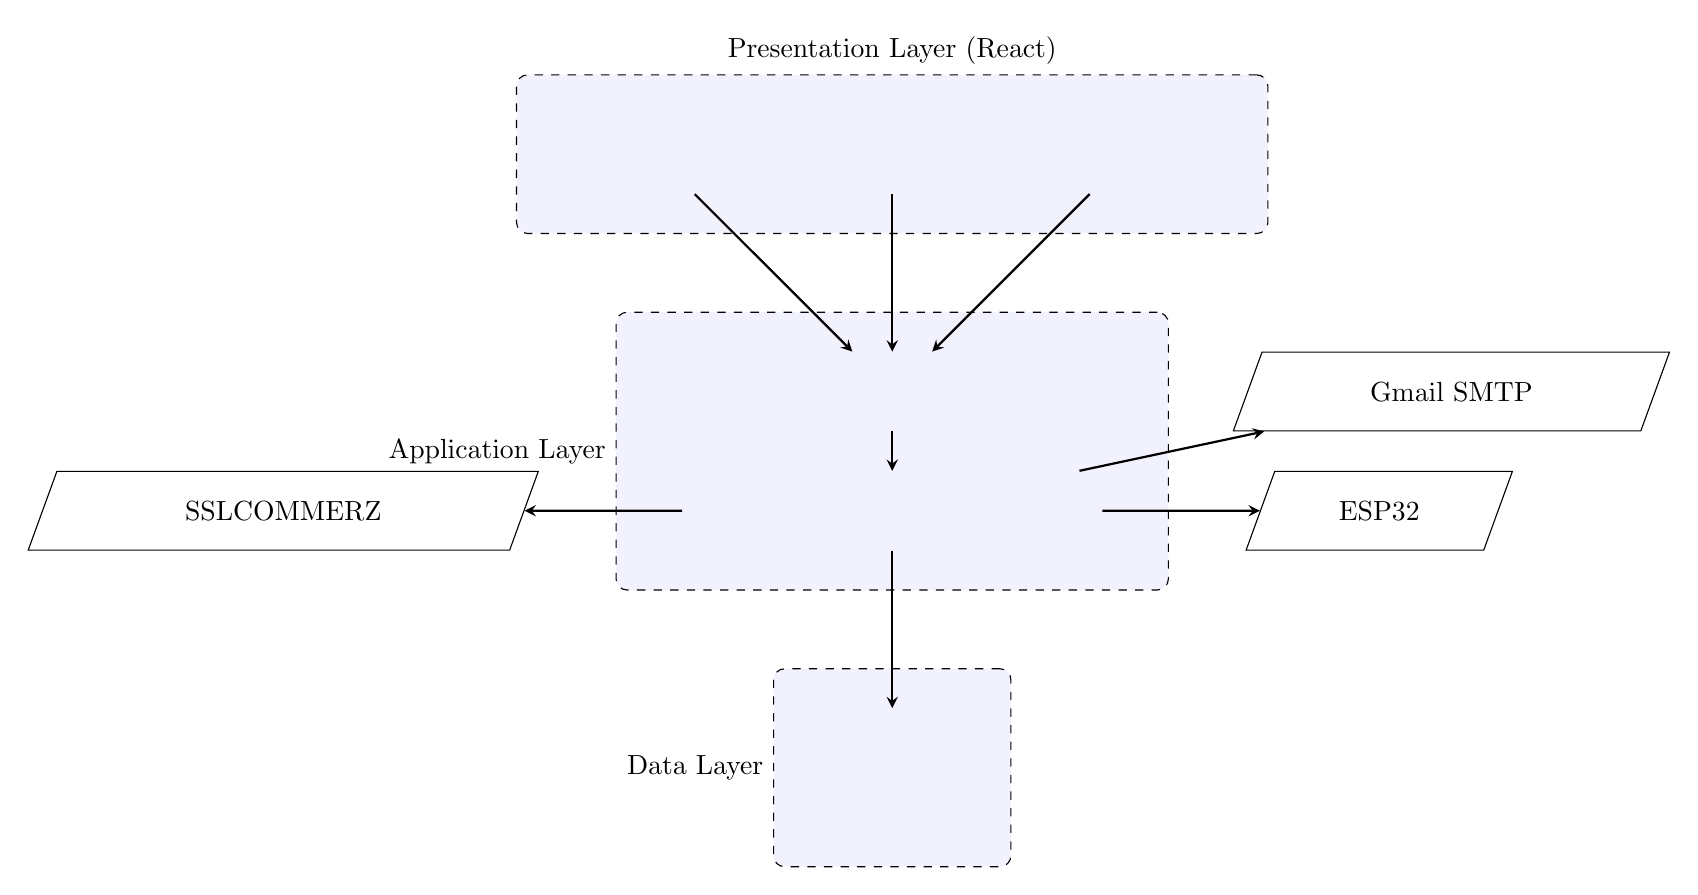
\begin{tikzpicture}[node distance=1.5cm]

% Presentation Layer
\node (student) [process] {Student Pages};
\node (admin) [process, right=0.5cm of student] {Admin Pages};
\node (auth) [process, right=0.5cm of admin] {Auth Pages};

\node[layer, fit=(student) (admin) (auth), label=above:Presentation Layer (React)] (presentation) {};

% Application Layer
\node (api) [process, below=2cm of admin, minimum width=6cm] {ASP.NET Core 8 Web API};
\node (services) [process, below=0.5cm of api] {Services (Auth, Payment, Email)};

\node[layer, fit=(api) (services), label=left:Application Layer] (application) {};

% Data Layer
\node (db) [database, below=2cm of services, minimum width=2cm, minimum height=1.5cm] {SQL Server};
\node[layer, fit=(db), label=left:Data Layer] (data) {};

% External
\node (ssl) [io, left=2cm of services] {SSLCOMMERZ};
\node (esp) [io, right=2cm of services] {ESP32};
\node (smtp) [io, right=of api] {Gmail SMTP};

% Connections
\draw [arrow] (student) -- (api);
\draw [arrow] (admin) -- (api);
\draw [arrow] (auth) -- (api);

\draw [arrow] (services) -- (db);
\draw [arrow] (api) -- (services);

\draw [arrow] (services) -- (ssl);
\draw [arrow] (services) -- (esp);
\draw [arrow] (services) -- (smtp);

\end{tikzpicture}
}
\caption{HDMS System Architecture}
\end{figure}

\section{Component Responsibilities}

\subsection{Presentation Layer (Frontend)}
\begin{longtable}{@{}ll@{}}
\toprule
\textbf{Component} & \textbf{Responsibility} \\ \midrule
\textbf{Student Pages} & Dashboard, token purchase, wallet, marketplace, feedback \\
\textbf{Admin Pages} & Dashboard, QR scanning, menu management, reports \\
\textbf{Auth Pages} & Login, registration, password reset \\
\textbf{Shared Components} & Layout, navbar, buttons, cards, forms \\
\textbf{API Module} & Axios client with JWT interceptors \\ \bottomrule
\end{longtable}

\subsection{Application Layer (Backend)}
\begin{longtable}{@{}ll@{}}
\toprule
\textbf{Component} & \textbf{Responsibility} \\ \midrule
\textbf{Controllers} & Handle HTTP requests, input validation, response formatting \\
\textbf{Services} & Business logic, external service integration \\
\textbf{Middleware} & Authentication, suspension check, CORS \\
\textbf{DTOs} & Data transfer objects for API contracts \\ \bottomrule
\end{longtable}

\chapter{Technology Stack}

\section{Backend Technologies}
\subsection{Framework \& Runtime}
\begin{tabular}{lll}
\toprule
\textbf{Technology} & \textbf{Version} & \textbf{Purpose} \\ \midrule
\textbf{.NET} & 8.0 & Runtime platform \\
\textbf{ASP.NET Core} & 8.0 & Web API framework \\
\textbf{C\#} & 12 & Programming language \\ \bottomrule
\end{tabular}

\subsection{NuGet Packages}
\begin{itemize}
    \item \texttt{Microsoft.EntityFrameworkCore.SqlServer}: SQL Server provider
    \item \texttt{Microsoft.AspNetCore.Identity.EntityFrameworkCore}: Identity management
    \item \texttt{Microsoft.AspNetCore.Authentication.JwtBearer}: JWT authentication
    \item \texttt{MailKit}: Email sending (SMTP)
    \item \texttt{QRCoder}: QR code generation
    \item \texttt{Swashbuckle.AspNetCore}: API documentation
\end{itemize}

\section{Frontend Technologies}
\subsection{Core Framework}
\begin{tabular}{lll}
\toprule
\textbf{Technology} & \textbf{Version} & \textbf{Purpose} \\ \midrule
\textbf{React} & 18.3.1 & UI framework \\
\textbf{Vite} & 5.4.10 & Build tool \\
\textbf{JavaScript} & ES2022+ & Language \\ \bottomrule
\end{tabular}

\subsection{NPM Packages}
\begin{itemize}
    \item \texttt{react-router-dom}: Client-side routing
    \item \texttt{axios}: HTTP client
    \item \texttt{html5-qrcode}: QR code scanning
\end{itemize}

\section{Hardware}
\begin{itemize}
    \item \textbf{ESP32}: Microcontroller for gate/conveyor control
    \item \textbf{Servo Motor}: Gate mechanism
    \item \textbf{IR Sensor}: Bowl detection
    \item \textbf{L298N}: Motor driver
\end{itemize}

\chapter{Database Schema}

\section{Entity Relationship Diagram}

\begin{figure}[H]
\centering
\resizebox{0.95\textwidth}{!}{
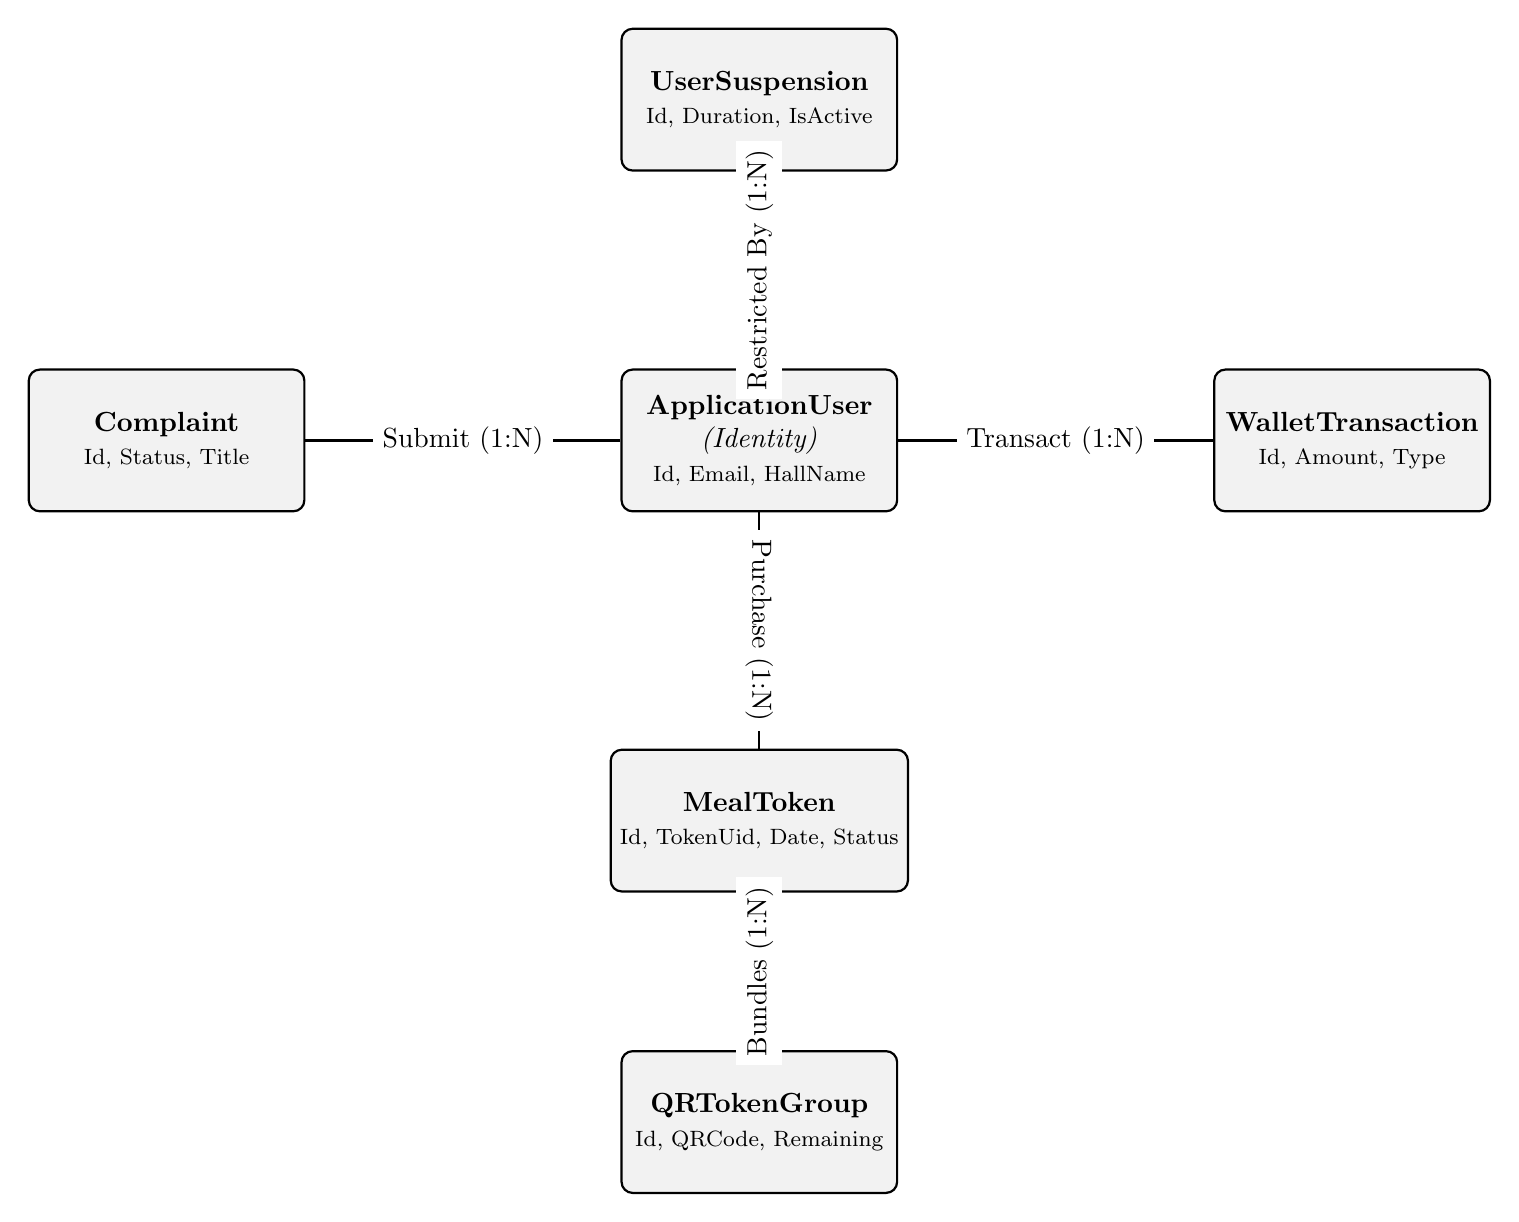
\begin{tikzpicture}[
    node distance=3cm,
    entity/.style={rectangle, draw=black, thick, fill=gray!10, minimum width=3.5cm, minimum height=1.8cm, align=center, rounded corners},
    relation/.style={diamond, draw=black, thick, fill=white, aspect=2, minimum width=2cm, align=center, font=\small},
    link/.style={thick, -}
]

% Nodes
\node (user) [entity] {\textbf{ApplicationUser}\\ \textit{(Identity)}\\ \footnotesize Id, Email, HallName};
\node (token) [entity, below=3cm of user] {\textbf{MealToken}\\ \footnotesize Id, TokenUid, Date, Status};
\node (wallet) [entity, right=4cm of user] {\textbf{WalletTransaction}\\ \footnotesize Id, Amount, Type};
\node (complaint) [entity, left=4cm of user] {\textbf{Complaint}\\ \footnotesize Id, Status, Title};
\node (suspension) [entity, above=2.5cm of user] {\textbf{UserSuspension}\\ \footnotesize Id, Duration, IsActive};
\node (group) [entity, below=2cm of token] {\textbf{QRTokenGroup}\\ \footnotesize Id, QRCode, Remaining};

% Edges
\draw [link] (user) -- node[pos=0.5, sloped, fill=white] {Purchase (1:N)} (token);
\draw [link] (user) -- node[pos=0.5, sloped, fill=white] {Transact (1:N)} (wallet);
\draw [link] (user) -- node[pos=0.5, sloped, fill=white] {Submit (1:N)} (complaint);
\draw [link] (user) -- node[pos=0.5, sloped, fill=white] {Restricted By (1:N)} (suspension);
\draw [link] (group) -- node[pos=0.5, sloped, fill=white] {Bundles (1:N)} (token);

\end{tikzpicture}
}
\caption{Entity Relationship Diagram (ERD)}
\end{figure}

\section{Core Entities}

\subsection{ApplicationUser}
\begin{lstlisting}[language=csharp]
public class ApplicationUser : IdentityUser
{
    public string FullName { get; set; } = string.Empty;
    public string StudentIdNumber { get; set; } = string.Empty;
    public string UserCode { get; set; } = string.Empty;  // MMHxxxxxx
    public decimal WalletBalance { get; set; } = 0m;
    // ... other properties
}
\end{lstlisting}

\subsection{MealToken}
\begin{lstlisting}[language=csharp]
public class MealToken
{
    public int Id { get; set; }
    public Guid TokenUid { get; set; } 
    public string StudentId { get; set; }
    public DateTime Date { get; set; }
    public MealType MealType { get; set; } // Lunch=1, Dinner=2
    public TokenStatus Status { get; set; }
    public DateTime? RedeemedAt { get; set; }
}
\end{lstlisting}

\subsection{WalletTransaction}
\begin{lstlisting}[language=csharp]
public class WalletTransaction
{
    public int Id { get; set; }
    public string UserId { get; set; }
    public decimal Amount { get; set; } // +Credit, -Debit
    public string Type { get; set; }    // TOPUP, PURCHASE, SALE
    public DateTime CreatedAt { get; set; }
}
\end{lstlisting}

\chapter{API Reference}

\section{Authentication}
\begin{itemize}
    \item \textbf{POST} \texttt{/api/auth/register}: Register new student
    \item \textbf{POST} \texttt{/api/auth/login}: Authenticate and get JWT
    \item \textbf{GET} \texttt{/api/auth/profile}: Get user details
\end{itemize}

\section{Tokens}
\begin{itemize}
    \item \textbf{GET} \texttt{/api/tokens/my}: List owned tokens
    \item \textbf{POST} \texttt{/api/tokens/redeem}: Admin redeem token (scan)
    \item \textbf{POST} \texttt{/api/orders/buy}: Purchase token
    \item \textbf{POST} \texttt{/api/orders/buy-qr-group}: Bulk purchase
\end{itemize}

\section{Marketplace}
\begin{itemize}
    \item \textbf{GET} \texttt{/api/marketplace/listings}: View internal market
    \item \textbf{POST} \texttt{/api/marketplace/listings}: Create listing
    \item \textbf{POST} \texttt{/api/marketplace/buy/\{id\}}: Buy from market
\end{itemize}

\chapter{Core Features}

\section{Digital Meal Tokens}
The core unit of the system. Tokens follow this lifecycle:
\begin{center}
\texttt{PURCHASED} $\rightarrow$ \texttt{LISTED} $\rightarrow$ \texttt{SOLD} $\rightarrow$ \texttt{REDEEMED}
\end{center}
Tokens can strictly only be redeemed on their specific date and meal time.

\section{QR Token Groups}
Allows students to buy 2-4 tokens at once (guest meals), generating a single QR code. The system tracks \texttt{RemainingTokens} for the group ID.

\section{Wallet System}
A closed-loop wallet system. Students top up via SSLCOMMERZ gateway.
\begin{itemize}
    \item \textbf{Top Up}: Online payment $\rightarrow$ Balance credit
    \item \textbf{Purchase}: Balance debit $\rightarrow$ Token created
    \item \textbf{P2P Sale}: Buyer debit $\rightarrow$ Seller credit
\end{itemize}

\section{AI Abuse Detection}
The system monitors complaint behavior to detect abuse.
\begin{itemize}
    \item \textbf{Metric}: Frequency of complaints (24h/7d)
    \item \textbf{Metric}: Content duplication (Levenshtein distance)
    \item \textbf{Action}: Auto-calc abuse score. If $>70$, auto-suspend user.
\end{itemize}

\chapter{Hardware Integration}

\section{ESP32 Controller}
The ESP32 microcontroller manages the physical entry gate.

\subsection{Wiring}
\begin{itemize}
    \item \textbf{GPIO 5}: Servo Signal
    \item \textbf{GPIO 4}: IR Sensor
    \item \textbf{GPIO 16/17}: L298N Motor Driver
\end{itemize}

\subsection{Flow}
\begin{enumerate}
    \item Admin scans QR in Frontend
    \item Backend validates token $\rightarrow$ Success
    \item Frontend calls ESP32 \texttt{/open-gate}
    \item ESP32 rotates servo 90 degrees for 5 seconds
\end{enumerate}

\chapter{Installation \& Setup}

\section{Prerequisites}
\begin{itemize}
    \item Node.js 18+
    \item .NET 8 SDK
    \item SQL Server 2019+
\end{itemize}

\section{Backend Setup}
\begin{lstlisting}[language=bash]
cd Hdms.Api
dotnet restore
dotnet ef database update
dotnet run
\end{lstlisting}

\section{Frontend Setup}
\begin{lstlisting}[language=bash]
cd hdms-client
npm install
npm run dev
\end{lstlisting}

\section{Configuration}
Ensure \texttt{appsettings.json} has valid connection strings and JWT secrets.
\begin{lstlisting}[language=json]
{
  "ConnectionStrings": {
    "DefaultConnection": "Server=...;Database=HdmsDb;..."
  },
  "Jwt": {
    "Key": "Minimum32CharactersLongSecretKey..."
  }
}
\end{lstlisting}

\end{document}
